\chapter{Решение на основе \texttt{Moflow gentrace}}

\section{Устройство оригинального инструмента}

Прежде всего, следует подробнее разобраться как устроен и работает \texttt{gentrace}. Для начала, на примере где все работает корректно.

Пусть некоторый файл был отмечен как источник помеченных данных, тогда при первом чтении этого файла при помощи системного вызова \texttt{read(fd, buf, 10)} будут созданы метки с номерами от $1$ до $10$ и поставлены в соответствие ячейкам памяти $\texttt{buf[0]}\ldots \texttt{buf[10]}$ соответственно. Пусть затем была выполнена инструкция \texttt{cmp rax, [buf+0x9]}, регистр \texttt{RFLAGS} становится помеченным меткой $10$, соответственно следующий условный переход зависит от $10$ого байта.


\begin{figure}[H]
    \center{
        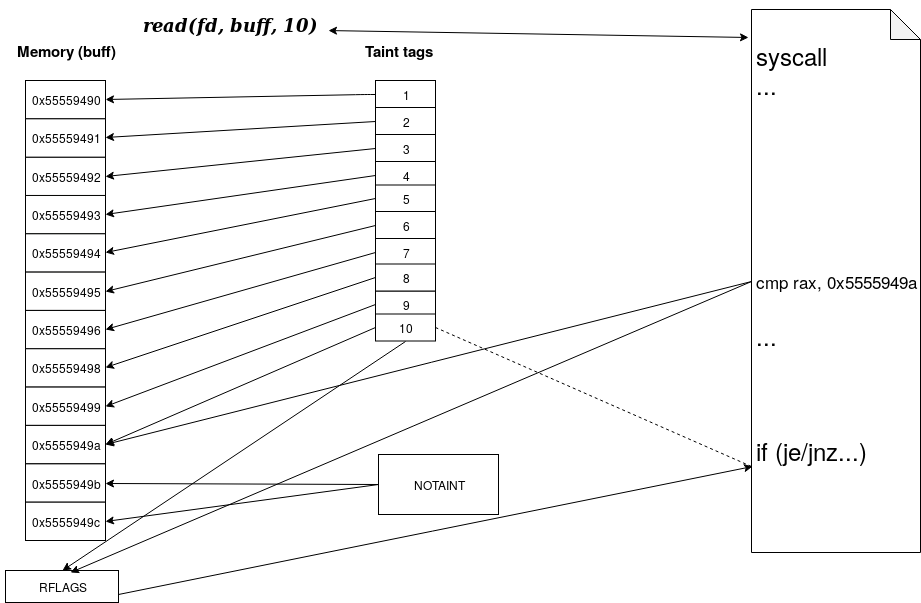
\includegraphics[scale=0.5]{img/source_tainting.png}
    }
    \caption{Создание пометок в \texttt{moflow gentrace}}
    \label{fig:moflow1}
\end{figure}

Теперь рассмотрим другой случай. Пусть после вызова \texttt{read(fd, buf, 10)} последует инструкция \texttt{mov rcx, qword ptr [rsi]}, где \texttt{rsi} хранит адрес \texttt{buf}. В то время как в действительности произошло побайтовое копирование, \texttt{moflow} видит это иначе.

\begin{itemize}
    \item Для каждого адреса или регистра, который читается в рамках инструкции берется соответствующая ему метка. Все полученные метки объединяются при помощи функции \texttt{combineTaint}.
    \item В каждый адрес или регистр, в которых во время инструкции происходит запись пишется метка, полученная в предыдущем пункте.
\end{itemize}

\begin{lstlisting}[environoment=cpp_code,captionpos=b]
uint32_t TaintTracker::combineTaint(uint32_t oldtag, uint32_t newtag)
{
  if (newtag) {// its tainted
    if (oldtag == NOTAINT)
      return newtag; // FIXME
    else 
      return MIXED_TAINT;
  }
  return oldtag;
}
\end{lstlisting}

Где \texttt{NOTAINT} это $0$ -- значение обозначающее, что метка отсутствует, а \texttt{MIXED\_TAINT} это $2^{32}-1$, обозначающее наличие более чем одной пометки.

\begin{figure}[H]
    \center{
        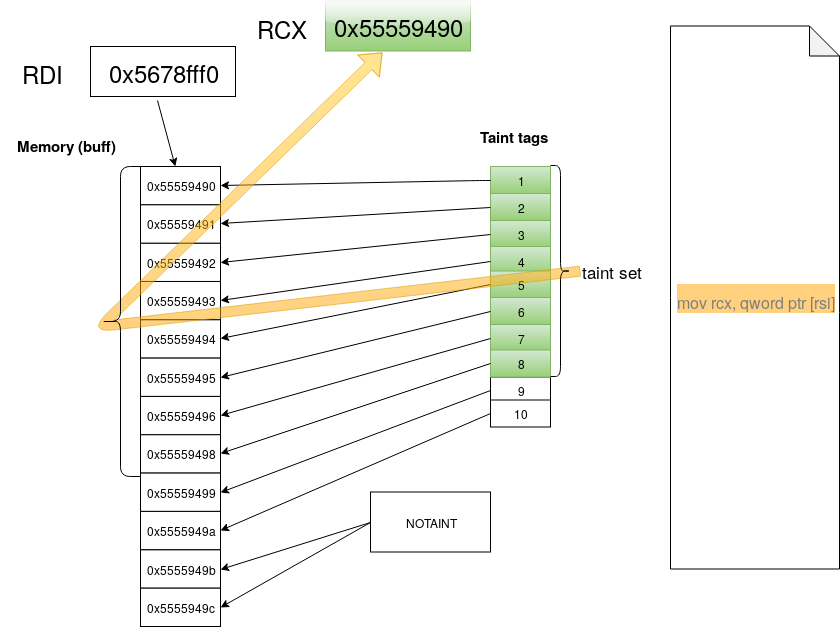
\includegraphics[scale=0.5]{img/propagation1.png}
    }
    \caption{Распространение пометок в \texttt{moflow gentrace}}
    \label{fig:moflow2}
\end{figure}

Таким образом, первое что необходимо реализовать это структуру \texttt{Множество меток}, которая должна поддерживать $3$ операции.

\begin{itemize}
    \item Добавление метки в \texttt{множество меток}.
    \item Объединение с другим \texttt{множество меток}
    \item Вывод содержимого Множества \texttt{множества меток}
\end{itemize}

Предположим теперь, что эта структура уже есть (далее будут описана её реализация). Допустим, встретилась еще одна инструкция копирования \texttt{mov word ptr [rdi], rcx}. \textbf{0x5678fff0} и \textbf{0x5678fff1}помечаются $8$ тегами. Правильно было бы представить \textbf{RCX} как 8 отдельных байт, которые могут быть помечены независимо, тогда \textbf{0x5678fff0} и \textbf{0x5678fff1} будут помечены $2$ различными тегами.

\begin{figure}[H]
    \center{
        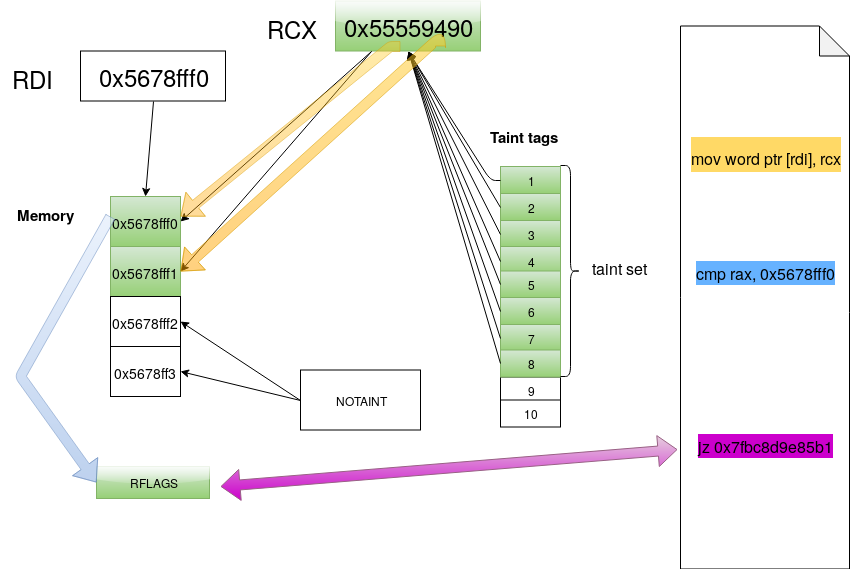
\includegraphics[scale=0.5]{img/propagation2.png}
    }
    \caption{Перепомечивание в \texttt{moflow gentrace}}
    \label{fig:moflow3}
\end{figure}

\section{Реализация \texttt{Множества Пометок}}

Наиболее простым и естественным решением, было бы использовать структуру данных реализующую интерфейс обычного множества в математическом смысле, в случае \texttt{C++} такой структурой данных является \texttt{std::set}. Тем не менее, непосредственные попытки использования вызвали ощутимые проблемы в производительности. Профилирование показало, что проблема в многочисленных аллокациях памяти, связанных c

\begin{itemize}
    \item Операцией объединения множеств
    \item Многочисленными аллокациями, вызванными необходимостью создавать временные множества пометок на каждую операцию распространения пометок
\end{itemize}

Дальнейший анализ показал, что на всех изученных примерах более чем в 70\% случаев соответствующие адресам и регистрам \texttt{множества пометок} оказываются пустыми или состоящими из одного элемента. Отсюда вытекает очевидная оптимизация. Будем представлять множество пометок в виде типа-суммы из двух элементов: \texttt{uint32\_t} и \texttt{tag\_set*}, где первый элемент используется как в оригинальном \texttt{gentrace}, то есть говорит об отсутствии метки, наличии единственной метки (в этом случае содержит её значение) или показывает, что меток более чем одна. В последнем случае используется непосредственно \texttt{tag\_set*}, в иных случаях значением второго элемента является нулевой указатель.

Не смотря на приведенную выше оптимизацию, остаётся необходимость реализовать структуру реализующую само множество. Были рассмотрены следующие варианты его реализации:


\subsection{Динамический массив}

В данной реализации был использован \texttt{std::vector} из стандартной библиотеки \texttt{C++}. При этом 
\begin{itemize}
    \item Добавлению соответствует операция добавления элемента в конец вектора.
    \item Объединению запись второго вектора в конец первого, с последующим удалением дублирующих элементов\footnote{Были проведены эксперименты, для определения границы при превышение которой стоит начать удаление дублей. Результаты показали, что разница между порогом в 20 элементов и меньшими статистически не различима, в то время как большие значение показывают худший результат}
    \item Вывод значений производится итерацией по элементам вектора.
\end{itemize}

\subsection{Битовое множество фиксированного размера}

Использование битового множества, представляется достаточно логичным решением, поскольку это структура данных, позволяющая быстро выполнить объединение множеств за линейное время -- операция сводится к выполнению побитового или, для этой операции также можно использовать \text{SSE} инструкции, что также положительно сказывается на производительности. Другим его преимуществом является компактность для хранения достаточно больших множеств, так $1$ байт может хранить информацию о $8$ метках.

Недостатком является объем занимаемой памяти, кроме того объединение множеств из $2$ элементов занимает столь же много времени, как и объединение множеств максимального поддерживаемого размера. Таким образом, эта структура данных может быть достаточно эффективна, если приходится оперировать достаточно большими множествами или если количество используемых меток невелико. Однако в ситуации когда меток много, причем конкретные адреса помечены их небольшим количеством -- битовое множество оказывается уже не столь эффективной структурой.

В стандартной библиотеке присутствует только реализация битового множества фиксированного размера \texttt{std::bitset}. Поскольку количество элементов должно быть известно на этапе компиляции, этот подход в чистом виде не применим. Тем не менее он представляет интерес как некоторый ориентир, в тестах было использовано значение в $6000$, как наименьшее круглое значение которого достаточно для тестовых примеров.
При данном подходе для всех операций использовался естественный интерфейс битового множества.

В библиотеке \texttt{Boost} есть реализация такой структуры данных как \texttt{dynamic\_bitset}, которая позволяет устанавливать размер множества динамически, а также менять его. Тем не менее, это решает только проблему с необходимостью знать количество меток на этапе компиляции. Все остальные проблемы остаются актуальными.

\subsection{Использование сжатых битовых векторов}

Использование сжатие для битовых векторов, потенциально позволяет решить проблему с достаточно разряженными битовыми векторами, и эффективно хранить множества с малым количеством меток.
В такой структуры данных было принято решение использовать библиотеку \texttt{CRoaring} -- реализацию протокола сжатых битовых векторов \texttt{Roaring} \cite{Roaring}. Данная библиотека в целом аналогична обычному битовому множеству с точки зрения интерфейса, однако поддерживает операции над множествами разного размера. Реализация также использовала естественный интерфейс множества, предлагаемый библиотекой.


\subsection{Ассоциативный массив битовых множеств}

Основным недостатком битового множества является необходимость хранить множество пустых битов на отсутствующие элементы, а преимуществом - возможность очень быстрой операции объединения. Один из подходов, позволяющих избавиться от этого недостатка был рассмотрен в предыдущем пункте, другой основан на следующей идее.

Будем использовать ассоциативный массив (\texttt{std::map} из стандартной библиотеки), ключами которого являются целые числа, а значениями битовые вектора размера $N$. Пусть \texttt{T} описанный ассоциативный массив, рассмотрим реализацию операций, которые он должен поддерживать.


\begin{itemize}
    \item \texttt{Добавление элемента}. Пусть в \texttt{T} следует добавить элемент $x$. Возможны 2 случая
    \begin{itemize}
        \item \texttt{T} не содержит элемента с ключом $\floor*{\frac{x}{N}}$. Тогда в \texttt{T} добавляется элемент с соответствующим ключом и битовым вектором из нулей в качестве значения, затем элемент с номером $x \bmod N$ этом битовом векторе устанавливается в $1$.
        \item \texttt{T} содержит элемент с ключом $\floor*{\frac{x}{N}}$. Тогда у битового вектора, соответствующего этому ключу элемент c номером $x \bmod N$ устанавливается в $1$.
    \end{itemize}
    \item \texttt{Объединение множеств}. Пусть \texttt{T} следует объединить с $\texttt{T}_2$. Для элементов присутствующих и в $\texttt{T}_2$ и в \texttt{T} выполняется операция побитового или. Элементы, которые есть только в $\texttt{T}_2$ копируются в \texttt{T}.
    \item \texttt{Печать содержимого} производится естественным образом, совершается обход всего содержимого $T$, при этом если элемент $i$ в битовом векторе, соответствующем ключу $k$ установлен в $1$, то следует напечатать номер метки $k \cdot N + i$.
\end{itemize}

\subsection{Множество интервалов}

Существует еще один подход к реализации \texttt{множества меток}. Если некоторое множество состоит из последовательных чисел, то для его представления можно хранить только первый и последний элемент. Соответственно произвольное подмножества натуральных чисел можно представить как дизъюнктное объединение таких интервалов, где отдельно стоящие элементы представляются в виде пары из одинаковых чисел.

Использование подобной структуры имеет смысл в случае если обрабатываемые множества состоят из малого количества интервалов, что является достаточно разумным предположениям для помеченных данных.

В качестве реализации использовался модуль \texttt{boost::icl::interval\_set} из проекта \texttt{Boost}.


\subsection{Тестирование производительности различных реализаций}

Для тестирования производительности были использованы 4 различных приложения

\begin{itemize}
    \item \texttt{cmark} -- программа для преобразования markdown в html, написанная на \texttt{C}, входной файл из $3379$ байт, количество инструкций в трассе \numprint{608398}, количество операций над множествами меток \numprint{205273}.
    \item \texttt{file} -- инструмент из binutils, определяющий тип файла, входной файл содержит строку \texttt{``1123235235346436\textbackslash n''}, количество инструкций в трассе \numprint{14343775}, количество операций над множествами меток \numprint{23494644}.
    \item \texttt{jpeg} -- программа из набора \texttt{LAVA} \cite{LAVA} для обработки jpeg файлов, входной файл из $5770$ байт, количество инструкций в трассе \numprint{9043561}, количество операций над множествами меток \numprint{55839222}.
    \item \texttt{libyaml} -- программа из набора \texttt{LAVA} для обработки yaml файлов, входной файл из $5242$ байт, количество инструкций в трассе \numprint{11580028}, количество операций над множествами меток \numprint{11157748}
\end{itemize}

% \textbf{}\\
% \scalebox{0.8}{
\begin{table}[H]
    \caption{Время работы в секундах для различных реализаций} \label{tab:compare}
    \scalebox{0.8}{
    \begin{tabular}[]{@{}lllllllll@{}}
    \toprule
    & vanilla & vector & bitset6000 & roaring & bitset64 tree & bitset256
    tree & bitset512 tree & interval set \tabularnewline
    \midrule
    % \endhead
    cmark & 3.5s & 4.6s & 3.7s & 4.2s & 3.8s & 3.7s & 3.7s & 3.7s \tabularnewline
    file & 20.8s & 47s & 60s & 70s & 45.5s & 46s & 47s & 46s \tabularnewline
    libjpeg & 14.5s & 1762s & 49s & 378s & 307s & 108s & 80s & 165s \tabularnewline
    libyaml & 16.5s & 22.5s & 25s & 26s & 23.5s & 23.5s & 23.5s & 24s \tabularnewline
    \bottomrule
\end{tabular}}
\end{table}

Исходя из результатов в таблице \ref{tab:compare}, было принято решение остановиться на реализации с ассоциативным массивом с $256$ битным битовым вектором. Код реализующий описанную структуру можно найти в приложении \ref{tagsetimpl}.

\section{Другие доработки}

Помимо реализации множества пометок было проделано еще несколько усовершенствований \texttt{Moflow gentrace}.

\subsection{Удаление ненужного функционала}

Целью изначального инструмента было сохранение трасс выполнения в формате \texttt{protobuf}, однако с точки зрения решаемой задачи в этом нет никакого необходимости. Более того, профилирование показало, что сохранение трассы ухудшает производительность.


\begin{table}[H]
    \centering
    \caption{Время работы с сериализацией и без} \label{tab:compare2}
    % \scalebox{0.4}{
    \begin{tabular}[]{@{}lll@{}}
    \toprule
    & с сериализацией трассы & без сериализации трассы  \tabularnewline
    \midrule
    % \endhead
    cmark & 3.7s & 3.4s \tabularnewline
    file & 46s & 29s \tabularnewline
    libjpeg & 108s & 99s \tabularnewline
    libyaml & 23.5s & 22s \tabularnewline
    \bottomrule
\end{tabular}
\end{table}

Как видно из таблицы \ref{tab:compare2} производительность инструмента возросла. Из других преимуществ следует отметить упрощение кодовой базы, и возможность использовать версию \texttt{Pin 3.7} по причине отсутствия внешних зависимостей.

\subsection{Улучшения работы с помеченными данными}

В оригинальном инструменте не была реализована поддержка некоторых системных вызовов под операционной системой Linux. Была добавлена поддержка \testtt{pread64}, \texttt{socket} и \texttt{recvfrom}.

Также была реализована возможность указания произвольной гранулярности меток и возможность использовать разметку входного файла для помечивания. Остановимся на этих возможностях чуть подробнее. 
В пункте \ref{taintmethod} упоминалась возможность использования \texttt{afl-analyze}, чтобы определить семантику использования некоторых байтов входного файла. 

\begin{figure}[H]
    \center{
        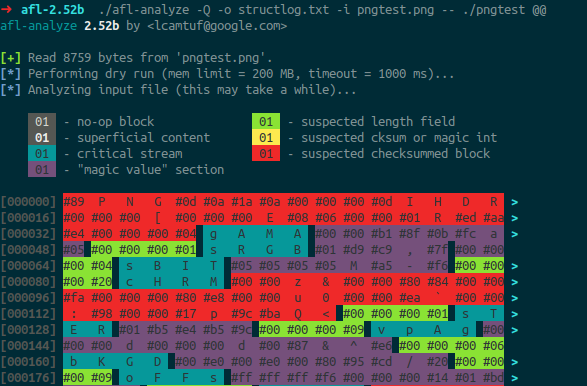
\includegraphics[scale=0.5]{img/afl-analyze.png}
    }
    \caption{Пример работы в \texttt{afl-analyze}}
    \label{fig:afl-analyze}
\end{figure}

На рисунке \ref{fig:afl-analyze} содержится пример результата работы этой утилиты. Был разработан вспомогательный инструмент на языке \texttt{Python}, обрабатывающий вывод \texttt{afl-analyze} c целью генерации json файла c информацией о разметке входного файла.

\texttt{Moflow gentrace} может использовать эту информацию как на рисунке \ref{fig:granularity}.
\begin{figure}[H]
    \center{
        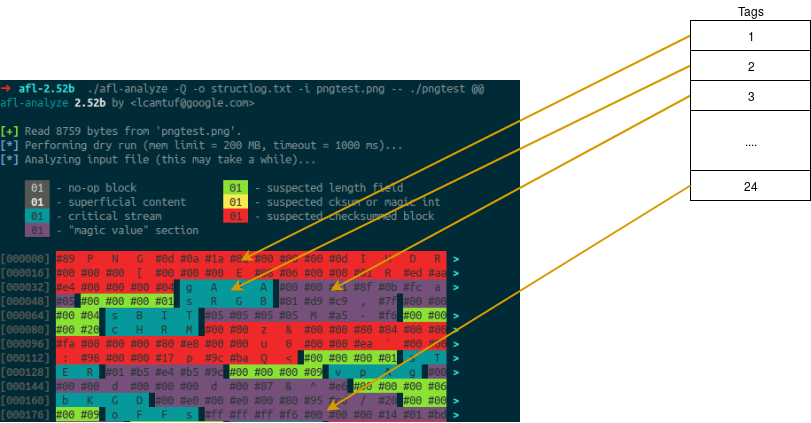
\includegraphics[scale=0.5]{img/granularity.png}
    }
    \caption{Помечевание основанное на выводе \texttt{afl-analyze}}
    \label{fig:granularity}
\end{figure}
Данные, для которых \texttt{afl-analyze} не смог определить семантику помечаются обычным образом.

Другой добавленной возможностью является указание грунулярности меток. Вместо того, чтобы ставить в соответствие каждому байту входных данных отдельную метку, была добавлена возможность использовать одну метку для $N$ последовательных байт. По умолчанию $N$ считается равным $1$, что соответствует обычной однобайтовой гранулярности.

Обе возможности могут использоваться одновременно.
